\chapter{Related Work}
\label{ch:RelatedWork}

Test-Driven Development (TDD), a core practice of Extreme Programming, 
has been widely adopted by software industry and studied by software 
engineering researchers. Industry practitioners have put increasing 
effort into evaluating and understanding TDD in recent years. Many books \cite{Beck:03,Astels:03,Newkirk:04,Link:03,Hunt:03} directly related 
to TDD have been published. XUnit\cite{XUnit,xUnitFrameWork}, the 
foundation of TDD, has been ported to more than 30 languages. Development 
tools such as Eclipse, NetBeans, and Visual Studio have been enhanced
to support unit testing, which makes it easier for practitioners 
to develop software in TDD. The community of TDD \cite{TestDrivenWeb,TddYahooGroup} 
is continuously growing, and some enthusiastic practitioners 
\cite{HawleyBlog,ExtremeJSBlog,MemoRandaBlog,EichertBlog,MasonBlog} 
even write about their personal experiences in their blogs. In addition 
to this industrial interest, software engineering researchers have 
begun studying TDD as an enabling software development method. Both 
pedagogical\cite{Muller:02,Edwards:04,Matjaz:03,Erdogmus:05,Kaufmann:03} 
and industrial \cite{George:03,Maximilien:03,Geras:04,Williams:03,Bhat:06} 
evaluations of TDD have been conducted in the last few years.  

So far, software engineering researchers have focused most of their 
energy on the outcomes that applying TDD brings to software products 
and software developers. However, compared to the claims made by 
practitioners, research findings of TDD on software quality and 
developer productivity are mixed. In fact, much of the research work on TDD 
suffers from the threat of ``construct validity'' \cite{Wang:04} 
because of the ``process conformance'' problem. Wang and Erdogmus define 
process conformance as ``the ability and willingness of subjects to follow 
a prescribed process''. Janzen and Saiedian warn that the inability to 
accurately characterize process conformance is harmful to TDD research, 
and that it is so hard to measure the usage of a development method 
such as TDD that current reports on adoption of TDD are not valid. 
Surveys are often used to measure the adoption of TDD, but only those 
who are much in favor or much opposed to it will respond. Janzen and 
Saiedian concluded that the combination of popularity of XP, JUnit 
and Eclipse likely implies a certain degree of adoption of TDD 
\cite{Janzen:05}. However, this is a very indirect measure.

Some of research work 
\cite{Cook:95,Jensen:05,csdl2-06-02,Wang:04,Wege:04} has been 
done on software process compliance using development activities 
and software artifacts collected from the development process. 
In my dissertation research, I focus on studying the process 
conformance of low-level software processes and Test-Driven 
Development in particular. 

Janzen claimed that TDD is a kind of software development method,
not a process model, and that it has emerged out of a particular 
set of process models \cite{Janzen:05}. In contrast, Beck and 
Cunningham, the pioneers of TDD, put it this way: ``test-first 
coding is not a testing technique but is rather about design.''
\cite{Beck:01} If TDD is a design technique and it drives the 
implementation of product code, then classifying it as a software 
process sounds reasonable. In my research, I have characterized
practices such as Test-Driven Development and Personal Software 
Process (PSP) as low-level software processes. A common 
characteristic of low-level software processes is that they are defined 
by many frequent and rapid short-duration activities. Unlike high-level 
and long duration phases such as ``requirement analysis'' that might 
last weeks to months, the activities in low-level software process 
such as ``refactor class Foo to extract interface IFoo'' may take 
only seconds to a few minutes \cite{csdl2-06-02}.

This chapter begins with a detailed introduction to TDD, followed 
by a discussion of TDD empirical studies.
The research results are mixed because of differences in experiment
settings, and the empirical studies suffer from construct validity
because of the process conformance problem of TDD. In the second
part, I present other related work on automated process conformance 
in contrast to my research that is built on the automated software 
metrics collection machinery of 
Hackystat \cite{Hackystat,csdl2-01-12,csdl2-01-13,csdl2-02-07}. 

\section{Test-Driven Development: A Short Introduction}
\label{sec:related-tdd}
\begin{quotation}
``\textit{Test-first coding isn't new. It's nearly as old as programming.}''

\raggedleft{--- Kent Beck}
\end{quotation}

\begin{comment}

Test-Driven Development\cite{Beck:03} is a software development practice
popularized by Extreme Programming \cite{Beck:00,Jeffries:00}. The key
characteristic of TDD is ``test-first'', in which developers should 
always write a test first according to the requirement, and then implement
the functional code to make the test pass. Because a test is always created 
first to drive the design and implementation, TDD used to be called Test-First 
Design (TFD) or Test-First Development (TFD) \cite{Beck:00}. 
\end{comment}

Test-Driven Development\cite{Beck:03} is a software development 
best practice popularized by Extreme Programming \cite{Jeffries:00,Beck:00}. 
It has two basic rules: ``(1) Write new code only if an automated test
has failed; (2) Eliminate duplication.''  Kent Beck, the pioneer of
Test-Driven Development, stated that there is an implicit order of 
programming in TDD \cite{Beck:03}: 
\begin{enumerate}
\item Red - Write a little test that does not work, and perhaps does not even
  compile at first.
\item Green - Make the test work quickly, committing whatever sins are
  necessary in the process.
\item Refactor - Eliminate all the duplication created by merely getting
  the test to work.
\end{enumerate}
The key characteristic of TDD is ``test-first'', with which developers 
should always write a test first according to the requirement, and then 
implement the functional code to make the test pass. Because a test is 
always created first to drive the design and implementation, TDD used 
to be called Test-First Design (TFD) or Test-First Development 
(TFD) \cite{Beck:00}. My opinion is that ``test first'' is better 
than ``test driven'' with respect to describing the order of test and 
production coding activities. Therefore, in the rest of this document, 
I will use ``test first'' when it is necessary to emphasize the order of 
programming in TDD, otherwise there is no difference between ``test first''
and ``test driven''.

Test first is as old as programming, and has been used for decades
 \cite{Williams:03,Beck:00,Beck:01}. Beck recalled that his first 
programming experience was actually in test-first using output and
input tapes \cite{Beck:01}. Indebted to the philosophy and popularity 
of Extreme Programming (XP), Test-Driven Development has emerged as a 
notable best practice for software development 
\cite{Beck:00,Jeffries:00}.

XP is a light weight software development methodology that is intended
for use when confronted by vague and rapidly changing requirements 
\cite{Beck:00}. It is rooted in observations on repeated best practices 
in software development. The philosophy of XP is to take common-sense 
principles and practices to an ``extreme'' level \cite{Beck:00,Jeffries:00}:
\begin{quote}
\begin{itemize}

\item If code reviews are good, we'll review code all the time (Pair Programming).

\item If testing is good, everybody will test all the time (unit testing), 
even the customers (Functional Testing).

\item If design is good, we will make it part of everybody's daily 
business (Refactoring).

\item If simplicity is good, we will always leave the system with 
the simplest design that supports its current functionality (the 
simplest thing that could possibly work).

\item If architecture is important, everybody will work defining and 
refining the architecture all the time (Metaphor).

\item If integration testing is good, then we will integrate and test 
several times a day (Continuous Integration).

\item If short iterations are good, we will make the iteration really, 
really short --- seconds and minutes and hours, not weeks and months and 
years (Planning Game).

\end{itemize}
\end{quote}

Figure \ref{fig:XPNetwork} illustrates the supporting network of twelve 
XP practices \cite{Beck:00}. 
\begin{figure}[htbp]
  \centering
  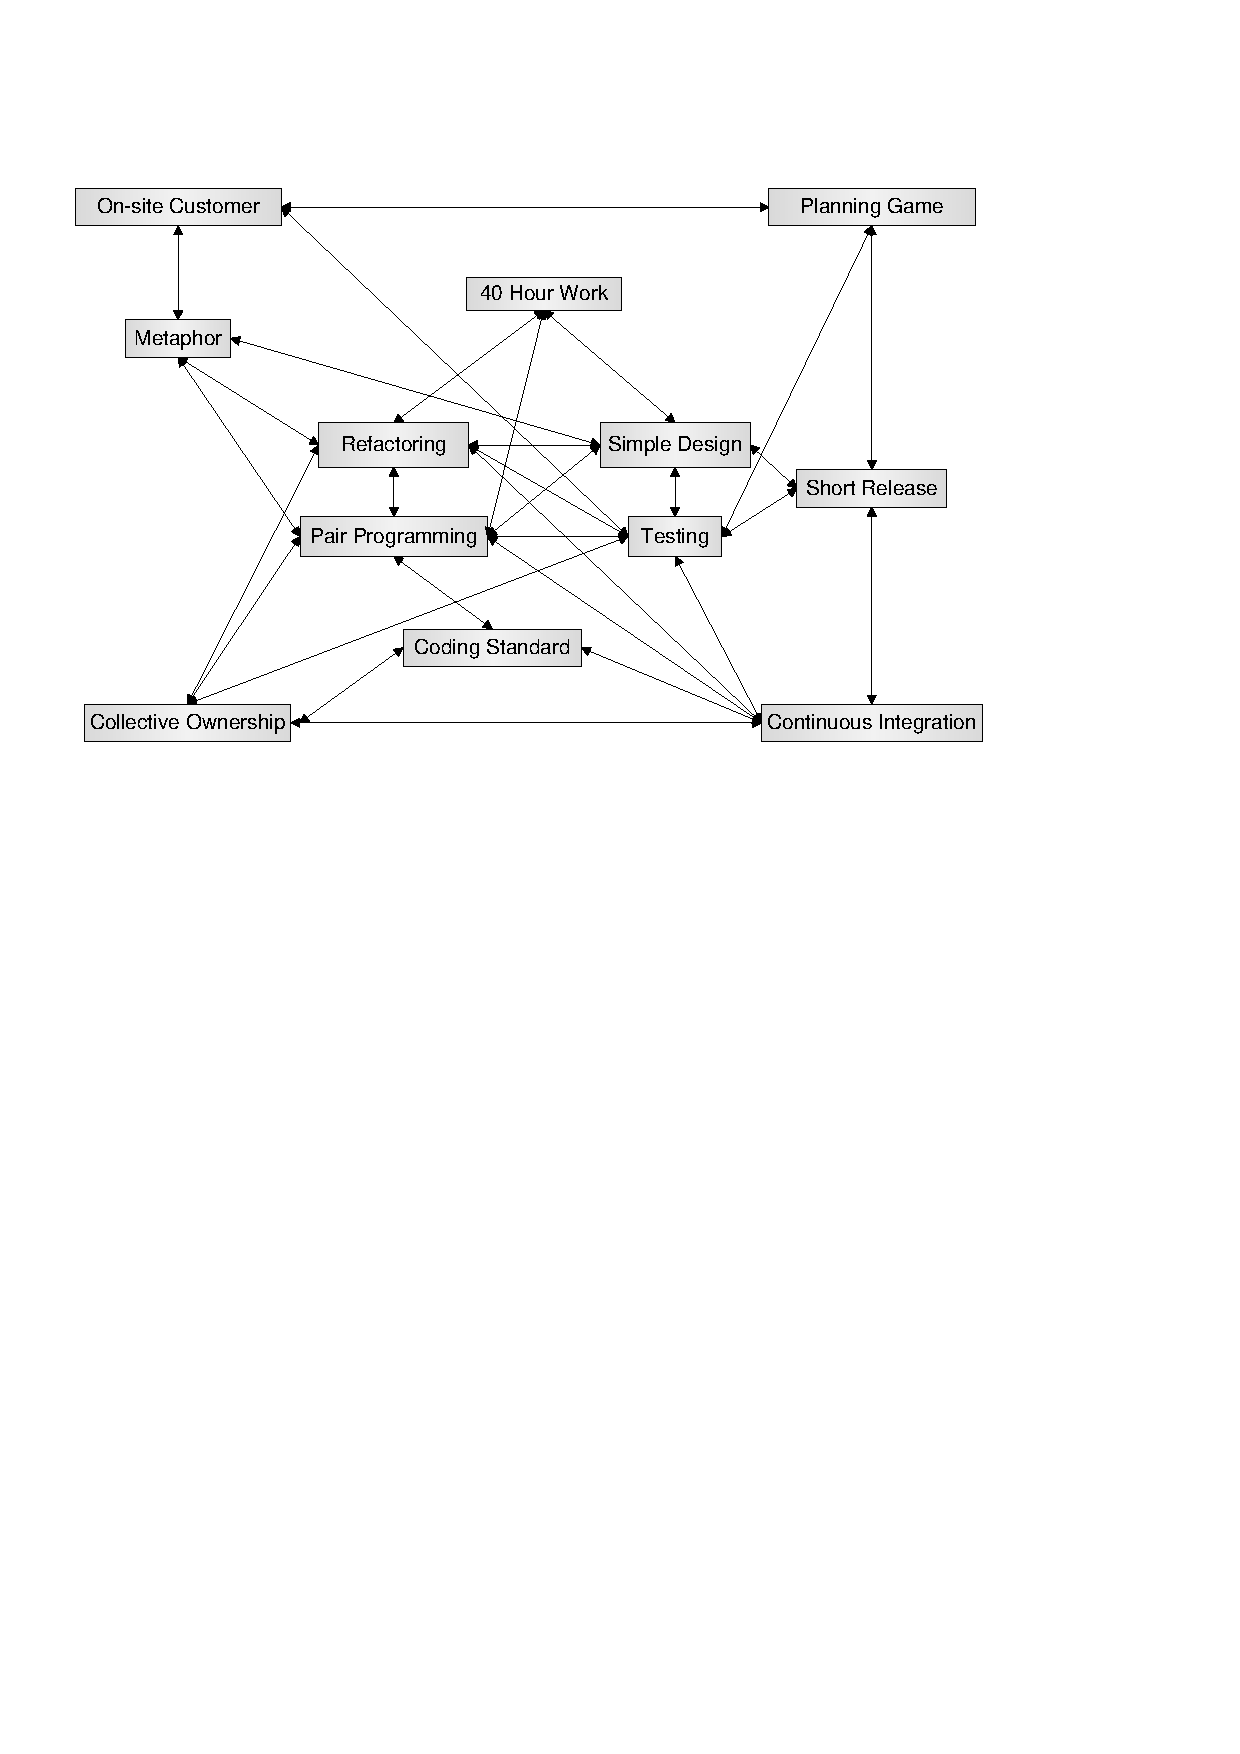
\includegraphics[width=0.6\textwidth]{figs/Visio-XPNetwork}
  \caption{Network of Extreme Programming Practices\cite{Beck:00}}
  \label{fig:XPNetwork}
\end{figure}
XP proposes TDD as the glue to hold the process together. TDD helps 
create a comprehensive suite of unit tests such that developers have 
the courage to consistently refactor code into a much simpler design.  

Though born as a practice of XP, TDD is often thought as an independent 
software development method. It can be used by practitioners and 
organizations that do not or partially practice XP 
\cite{Beck:03,TestDrivenWeb,TddYahooGroup}. Many TDD training workshops 
\cite{OsheroveWorkshop:04,ClarkwareWorkshop:04,
AdaptionTddWorkshop,IndustrialLogicTddWorkshop,TestDrivenDotComWeblogs,
BENUGWorkshop:04} have been provided by experienced practitioners 
and consulting companies. An informal 
survey \cite{UnitTestingPoll:06} conducted by the Method and 
Survey magazine found that 46\% of the studied software 
organizations perform unit testing informally, 41\% of the 
studied organizations document their unit test cases, and 
14\% of the studied organizations use the TDD approach.

\subsection{Characteristics of TDD}
\begin{quotation}
``\textit{Never write a line of functional code without a broken test case.}''

\raggedleft{--- Kent Beck}
\end{quotation}
\begin{quotation}
``\textit{Test first coding is not a testing technique.}'' 

\raggedleft{--- Ward Cunningham}
\end{quotation}

Recall that the two basic rules of TDD are to ``(1) Write new code 
only if an automated test has failed; (2) Eliminate duplication.''
Following the first rule, given a requirement, a TDD developer 
analyzes it first, and then outlines a To-Do list with a few tasks. 
The tasks can be very simple but should suffice to enable some 
development to occur. The developer can start a task that is either easy 
to do or essential to the problem to be solved 
\cite{Astels:03, Beck:03}. After picking a task, the developer 
writes a unit test first, and then invokes it. The test invocation 
might fail because it tests something that does not exist. The 
failing test drives the implementation of new functional code
to make it pass. Often, it is also necessary to run all tests to
make sure nothing is broken. The second rule is to eliminate
the duplication. If redundancy is introduced in the first
step, the developer should refactor either test code or functional
code to remove it. It is also necessary to run all tests 
after refactoring to confirm that nothing is broken. This 
is an iteration of TDD. A common belief is that TDD iterations 
should not last more than 10 minutes \cite{TDDRhythm}. 
After an iteration is over, the developer can cross out the
finished task from the To-Do list, and pick another task  
to begin a new iteration. Additionally, the developer should
add new tasks to the To-Do list whenever he or she wants. The 
characteristics of TDD are :
\subsubsection{Test First}
Test first is the key characteristic of TDD. Importantly, in 
TDD, developers should ``never write a line of functional 
code without a broken test case'' \cite{Beck:01}. 

\subsubsection{Short Iterations}
Quickly adding functional code to make test pass is important
to TDD. An iteration should last a few seconds to 
several minutes only. If hours of work is needed to make a 
test pass, probably the developer should divide the programming 
task into several sub tasks that can be solved in a shorter
period of time. 

\subsubsection{Frequent Refactoring}
Code is consistently refactored in TDD to create the simplest
possible design. The existence of a suite of unit tests gives 
developers the ``courage'' to refactor the code \cite{Beck:03}. 

\subsubsection{Rapid Feedback}
Unit testing is usually supported by the XUnit\cite{XUnit}
framework that is available in most mainstream languages. 
After new functional code is added, developers can invoke
the unit tests to test it right away. The feedback is available
within seconds or minutes. 

\subsubsection{One Ball in the Air at Once}
In typical software development, a developer usually carries 
a baggage with the requirement, system structure design, algorithm, 
code efficiency, readability and communication with other code 
etc. Martin Fowler described that the process is like keeping 
several balls in the air at once (Page 215 in \cite{Beck:03}), 
while the developer only keeps one ball in the air at once and 
concentrates on that ball properly in TDD. In the development
step, the developer only needs to make the test pass 
without worrying about whether it is a good or bad design. In 
the refactoring step, the developer only worries about what 
makes a good design. 

\subsubsection{Always Working Code}
The code should be always working in TDD because developers run 
all tests at the end of each iteration. If any test has failed, 
the developer should fix it right away. The fix should be easy because 
only a small amount of code is written in each iteration. If running 
all tests after an iteration is not feasible, the continuous 
integration can be set up to run them all once a day or several 
times a day. 

\subsection{Benefits of TDD to Software Development}

\begin{quotation}
``\textit{I have spent enough time in my career on silly 
bug-hunting, with TDD those days are gone. Yes, there are 
still bugs, but they are fewer and far less critical.}'' 
\cite{ExtremeJSBlog} 

\raggedleft{---Thomas Eyde}
\end{quotation}

The two most notable benefits of TDD are high quality
and developer productivity \cite{Beck:01,Janzen:05} :

\subsubsection{High Quality}
Probably the most advocated benefit of TDD is the high 
code quality. Because software quality is hard to measure, 
practitioners and researchers often use code coverage as 
the proxy of software quality. The code developed in TDD 
should be 100\% covered since no functional code is created 
without a unit test. 

\subsubsection{High Productivity}
Functional code and test code are both products. Testing is 
part of the design process, and it does not take a long time 
to write a small test. If developers need to write same amount 
of test code, TDD should save development time because less 
time is spent on tests than in the traditional test last or ad-hoc 
development methods. In addition, TDD users claim that the 
method reduces the overall amount of time spent on debugging, 
with a resulting increase in overall productivity\cite{Williams:03}.

% When and how TDD was developed
% Introduction to Extreme Programming
% XP and TDD are widely adopted in industry
% Benefit of TDD. Wide spread of TDD in the industry.
%
% Extensive research work has been conducted on Test-Driven Development

\section{TDD Research Work}
\label{sec:related-empirical}

Much research work has been conducted on studying important
outcomes of TDD such as software quality and developer productivity 
in recent years. In addition to anecdotal experience reports
\cite{George:04,Maximilien:03,Williams:03,Kaufmann:03,Edwards:04,Bhat:06}, 
researchers have run controlled experiments 
\cite{Muller:02,Matjaz:03,Erdogmus:05} to compare TDD against other 
development methods such as test last and ad hoc. Depending on whether
the test subjects are students or professional developers, the research
work can be categorized into academic and industrial studies.

\subsection{Empirical Evaluation in Academic Settings}

M\"{u}ller and Hanger \cite{Muller:02} conducted a study in an 
XP class in Germany to test TDD against traditional programming. 
The acceptance tests were provided 
to both the TDD group and the control group. Interestingly, students 
in the TDD group spent more time but their programs were less reliable 
than the control group.  

Edwards \cite{Edwards:04} adopted TDD in a junior-level class to compare
whether students got more reliable code after the use of TDD and WEB-CAT,
an assignment submission system. It turned out that the students using TDD
reduced their defect rate dramatically (45\% fewer defects/KSLOC using a
proxy metric) after adopting TDD, and a posttest survey found that TDD
students were more confident of the correctness and robustness of their
programs.

Similarly, Kaufmann and Janzen \cite{Kaufmann:03} conducted a pilot study 
on implications of TDD in an advanced project-oriented software 
engineering course. They also reported that TDD helped to improve software 
quality and programmers' confidence.

Pan\v{c}ur, Ciglari\v{c}, Trampu\v{s}, and Vidmar \cite{Matjaz:03} designed 
a controlled experiment to compare TDD with Iterative Test-Last approach 
(ITL), which is a slightly modified TDD development process in the order 
of ``code-test-refactor''.  This study
found that TDD is somewhat different from ITL but the difference is very
small. 

A more recent study on the effectiveness of TDD conducted by Erdogmus,
Morisio and Torchiano \cite{Erdogmus:05} used the well-defined test-last
and TDD approaches as Pan\v{c}ur did in \cite{Matjaz:03}. This study 
concluded that TDD programmers wrote more tests per unit of programming 
effort. More test code tends to increase software quality. Thus, TDD appears 
to improve the quality of software but TDD group in the study did not 
achieve better quality on average than test-last group. 

\subsection{Empirical Evaluation in Industrial Settings}
Several attempts have been made by researchers to study software quality
and developer productivity improvements of TDD in industrial settings.  

George and Williams \cite{George:04} ran a set of structured experiments
with 24 professional pair programmers in three companies. Each pair was
randomly assigned to a TDD group or a control group to develop a bowling
game application. The final projects were assessed at the end of the
experiment.  They found that TDD practice appears to yield code with
superior external code quality as measured by a set of blackbox test cases,
and TDD group passed 18\% more test cases. However, the TDD group spent
16\% more time on development, which could have indicated that achieving
higher quality requires some additional investment of time. Interestingly,
and in the contrast to the empirical findings, 78\% of the subjects
indicated that TDD practice would improve programmers' productivity.

Maximilien and Williams \cite{Maximilien:03} transitioned a software team
from an ad-hoc approach to testing to TDD unit testing practice at IBM, and
this team improved software quality by 50\% as measured by Functional
Verification Tests (FVT).

Williams, Maximilien, and Vouk \cite{Williams:03} conducted another case
study in IBM to study TDD. Compared to a baseline project developed in a 
traditional fashion, the defect density of the project developed 
in TDD was reduced by 40\% as measured by functional verification and 
regression tests. The productivity was not impacted by the additional 
focus on producing test code. 

Geras, Smith and Miller \cite{Geras:04} isolated TDD from other XP
practices, and investigated the impact of TDD on developer productivity and
software quality. In their research, TDD does not require more time but
developers in TDD group wrote more tests and executed them more frequently,
which may have led to future time savings on debugging and development.

Another study of TDD at Microsoft conducted by Bhat and Nagappan
\cite{Bhat:06} reported remarkable software quality improvement as 
measured in number of defects per KLOC. After introduction of TDD, 
project A (Windows) reduced its defects rate by 2.6 times, and project 
B (MSN) reduced its defect rate by 4.2 times, compared to the organizational
average. Reportedly, developers in project A spent 35\% more development
time, and developers in project B spent 15\% more development time, than
the developers in non-TDD projects spent.

\subsection{Discussion of Empirical Evaluation Studies}
The research findings of empirical studies are mixed on software quality 
and developer productivity as shown in Table \ref{tab:TDDResearchWork2}. 
The study conducted in Microsoft \cite{Bhat:06} and the study conducted 
in University of Karlsruhe \cite{Muller:02} are two extreme cases. In 
\cite{Bhat:06}, the developers improved software quality up to four 
times after adopting TDD. In comparison, the TDD group in \cite{Muller:02} 
yielded less reliable programs than the control group. In the following,
I will compare the research results according to the differences in
experiment settings. 

\begin{sidewaystable}[htbp]
\centering
  \begin{tabular}{|l|l|l|l|l|l|} \hline 
 & Investigator	& Study Type & Participants	& Software Quality	& Developer Productivity \\ \hline
 & George \cite{George:03} & Controlled Experiment	& 24	& TDD passed 18\% more tests & 16\% more time \\ \cline{2-6}
 & Geras \cite{Geras:04}  &  Controlled Experiment & 14	& TDD has the edge on quality & No impact \\ \cline{2-6}
 Industrial
 & Maximilien	\cite{Maximilien:03} & Case Study &  9	& 50\% reduction in defect density	& Minimal impact \\ \cline{2-6}
 & Williams\cite{Williams:03} & Case Study & 9	& 40\% reduction in defect density	& No change \\ \cline{2-6}
 & Bhat	\cite{Bhat:06}  & Case Study & 11	& 2-4 times reduction in defect density	& 35\% and 15\% more time \\ 
 
 \hline \hline
 
         & Kaufmann \cite{Kaufmann:03}	& Controlled Experiment &  8	& N/A	    & 50\% improvement \\ \cline{2-6}
         & Edwards \cite{Edwards:04} & Case Study & 59	& 54\% fewer defects	& N/A \\ \cline{2-6}
Academic & Erdogmus	\cite{Erdogmus:05} & Controlled Experiment & 35	& No change	  & Improved productivity \\ \cline{2-6}
         & M\"{u}ller \cite{Muller:02} & Controlled Experiment & 19 & Less reliable, but better reuse	& No change \\ \cline{2-6}
         & Pan\v{c}ur	\cite{Matjaz:03} & Controlled Experiment & 38	& No change	  & No change \\ \hline
  \end{tabular}
  \caption{Research Work of TDD on Software Quality and Developer Productivity}
  \label{tab:TDDResearchWork2}
\end{sidewaystable}


\subsubsection{Students vs. Professional Developers}
One difference is in population. The studies in academic settings 
used students as test subjects, while the studies in industrial 
settings recruited professional developers. 
Of 10 empirical studies listed in Table \ref{tab:TDDResearchWork2},
5 were conducted in academic settings, and the other 5 were 
conducted in industrial settings. The 
studies conducted in industrial settings found evidence of 
software quality improvements, but often at the cost of 
decrease of developer productivity. On the contrary, the 
studies in academic settings often found no software quality 
improvement but increase of developer productivity. 

How come the research findings are so divided among studies 
conducted within different population? Did professional 
developers pay more attention to software quality than 
students? Were students more concerned about productivity
than professional developers?  A caveat of industrial studies 
is that they must be beneficial to participants. 
In \cite{Maximilien:03}, Maximilien and Williams proposed TDD as 
a solution to reduce the defect rate. In \cite{Williams:03}, Williams,
Maximilien and Voulk assigned a dedicated coach to the development 
team. George and Williams \cite{George:03} noticed that the control 
group did not write worthwhile automated tests, partially due to the 
lack of incentives. Brilliant and Knight \cite{Brilliant:99} note 
that industry does not perceive a significant benefit from working 
with academic researchers in many cases. Researchers have to be able
to convince industry practitioners of the benefits and provide 
assistance in order to conduct research in industrial settings. 
The benefits are important to the participants of industrial studies, 
otherwise the quality of research would degrade. Geras, Smith and 
Miller reported that professional developers are hard to recruit 
when participation is voluntary \cite{Geras:04}. 

Students are generally less experienced at software development 
when compared to professional software developers. It is unclear 
whether students are appropriate participants for effectively
studying TDD \cite{Erdogmus:05}. M\"{u}ller and Hagner reported 
that the TDD group produced code with 74\% branch converage only, while the control 
group produced code with 80\% branch coverage \cite{Muller:02}. 
Erdogmus, Morisio and Torchiano \cite{Erdogmus:05} discussed 
the causal relationship between research findings and participant 
skill levels. They found that the students with high skill rate 
improved productivity more dramatically than the students with 
low skill rate. 

\subsubsection{Case Study vs. Controlled Experiment}
Another difference between the academic and industry based research
is in research methods. Case study and 
controlled experiment are the two most popular research methods. 
Of the 10 studies listed in Table \ref{tab:TDDResearchWork2}, 6 
are controlled experiments and 4 are case studies. Most of the
controlled experiments were conducted in academic settings because
classroom settings are more amenable to controlled experimentation. 
Since industry rarely repeats the same project twice, it is hard to have 
controlled experiments in industrial settings. Three out 
of five industrial studies were case studies. 

In controlled experiments, researchers often isolated test
first from TDD to compare it against other development 
methods such as test last and ad-hoc \cite{Muller:02,Matjaz:03,
Erdogmus:05,George:03,Geras:04}. Half of the controlled 
experiments \cite{George:03,Kaufmann:03,Erdogmus:05} observed 
productivity improvement in TDD groups, but only two studies 
found evidence of software quality improvement. On the contrary, 
the participants in the case studies improved software quality 
dramatically after adopting TDD, but they also spent more time 
on development.  

\subsubsection{Rivalry Development Methods}
The third difference of experiment settings is in the 
development methods that TDD was compared against. Researchers 
compared TDD against the traditional test-last\cite{Kaufmann:03,Geras:04}, 
ad hoc\cite{Muller:02,George:03}, and iterative test last 
(ITL) \cite{Matjaz:03,Erdogmus:05} methods. TDD did not help to 
improve software quality when it was compared against ITL. 
But it helped to improve software quality when it was compared 
with ad hoc and test last methods. Though TDD developers 
spent more development time, they also wrote more tests 
\cite{George:03,Erdogmus:05} and ran tests more frequently
\cite{Geras:04}.

\subsection{Process Conformance of TDD}
In the previous section, I have discussed the mixed research 
findings of TDD due to differences in population, research 
methods and the development methods that TDD was compared 
to. However, the research findings of studies in the same group  
were often consistent. For example, all the case studies found 
evidence of software quality improvement of TDD. Perhaps this 
phenomenon indicates that there are flaws in the empirical
studies of TDD. 

Erdogmus, Morisio and Torchiano \cite{Erdogmus:05} discussed that
a threat to the validity is ``process conformance'',
which is the level of conformance of the subjects
to the prescribed techniques. In order to improve process conformance,
they informed participants of the importance of following the 
proper procedures, and conducted a post test survey to filter 
unconformant data points\cite{Erdogmus:05}. Although they first
identified process conformance as a threat to the validity 
of research results of TDD, they were not alone in 
dealing with it. M\"uller and Hagner \cite{Muller:02} also 
indicated that their experiment was not technically controlled. 
During the experiment, they had to ask TDD groups if they were
following the test-first process. Pan\v{c}ur, Ciglari\v{c}, 
Trampu\v{s}, and Vidmar \cite{Matjaz:03} instrumented Eclipse, 
the development tool used in their study, to report unit test 
invocation frequency, results and time taken. A similar 
instrumentation method was used by Geras, Smith and Miller 
\cite{Geras:04}. However, instrumenting test invocation is 
a poor measure for process conformance of TDD because developers 
in test last groups can also run tests frequently. In 
\cite{George:03,Williams:03,Maximilien:03}, researchers studied 
test-first along with pair programming, which served as the 
process control method. Clearly, none of these methods is 
reliable at controlling participants' compliance to TDD or 
the rivalry development methods. 

Test first is a key characteristic of TDD, and developers 
should ``never write a line of functional code without a broken 
test case.'' \cite{Beck:01}. Short iterations, frequent 
refactoring, one ball in the air at once, and always working 
code are other characteristics of TDD. Developing software in 
TDD needs skills, practice, and discipline. On one hand, it is 
being widely adopted and embraced by software industry. Many 
developers simply enjoy the ``dance'' of test first and claim that
they are ``test-infected'', a phrase that is often used by the 
members of TDD community. On the other hand, the empirical research 
findings of TDD are often mixed. One of the causes of 
confused research results is the process conformance problem. 
In my thesis research, I have focussed on developing an automated 
machinery to evaluate the TDD conformance. Moreover, this work 
can be extended to study other low-level software processes as 
well. In a broader view, my work belongs to the research of automated 
software process. Some work has been conducted on this 
direction \cite{Cook:95,Cook:96,Jensen:04,Jensen:05}.

% We must collect low-level development behaviors in order
% to understand why TDD is employed and how it is used. 

\section{Automated Software Process Research}
\label{sec:related-automation}
Software process research is historically top-down. Process
programming\cite{Sutton:95}, modeling\cite{Curtis:92} and 
simulation\cite{Turnu:04,Jensen:05} are typical research 
methods for studying software processes. These top-down
methods are not usable for studying the process conformance of 
low-level software processes. They are appropriate when 
processes are confined and variations are very rare. 
However, these conditions are not easily met for low-level
software processes that define how developers should carry
on development activities at the granularity of minutes
and hours. Given a low-level software process, the actual 
process can be very different from the ideal process 
\cite{csdl-98-04,csdl2-06-01,csdl2-01-12}, which in turn leads 
to the issue of process conformance. 

In my research, I used a bottom-up research method. I applied 
rules on automatically gathered low-level development activities 
to infer the actual process, and compared the inferred process 
against the idealized process automatically, enabled by the 
rule-based system. My work is related to Cook's ``Automating 
Process Discovery and Validation'' and Jensen's ``Discovering 
and Modeling Open Source Software Processes'' because we all 
studied the automated evaluation of software processes using 
low-level development activities and software artifacts. 

%
% My thesis research focus is on designing an automated, 
% coherent framework to study the process conformance 
% of low-level software processes. 

\subsection{Automating Process Discovery and Validation}
Cook and Wolf \cite{Cook:95,Cook:96} developed a client-server 
system named Balboa to automate the process discovery using 
finite state machine (FSM). Balboa collects developers' 
invocations of Unix commands and CVS commits to construct
event streams. It then uses a neural network, a MARKOV chain, 
and data mining algorithms to discover 
the FSM of software processes. With Balboa, Cook and Wolf 
were able to reproduce the ISPW 6/7 process in their research. 
Figure \ref{fig:Balboa} illustrates the ISPW 6/7 process they 
discovered using the Markov Model.
\begin{figure}[htbp]
  \centering
  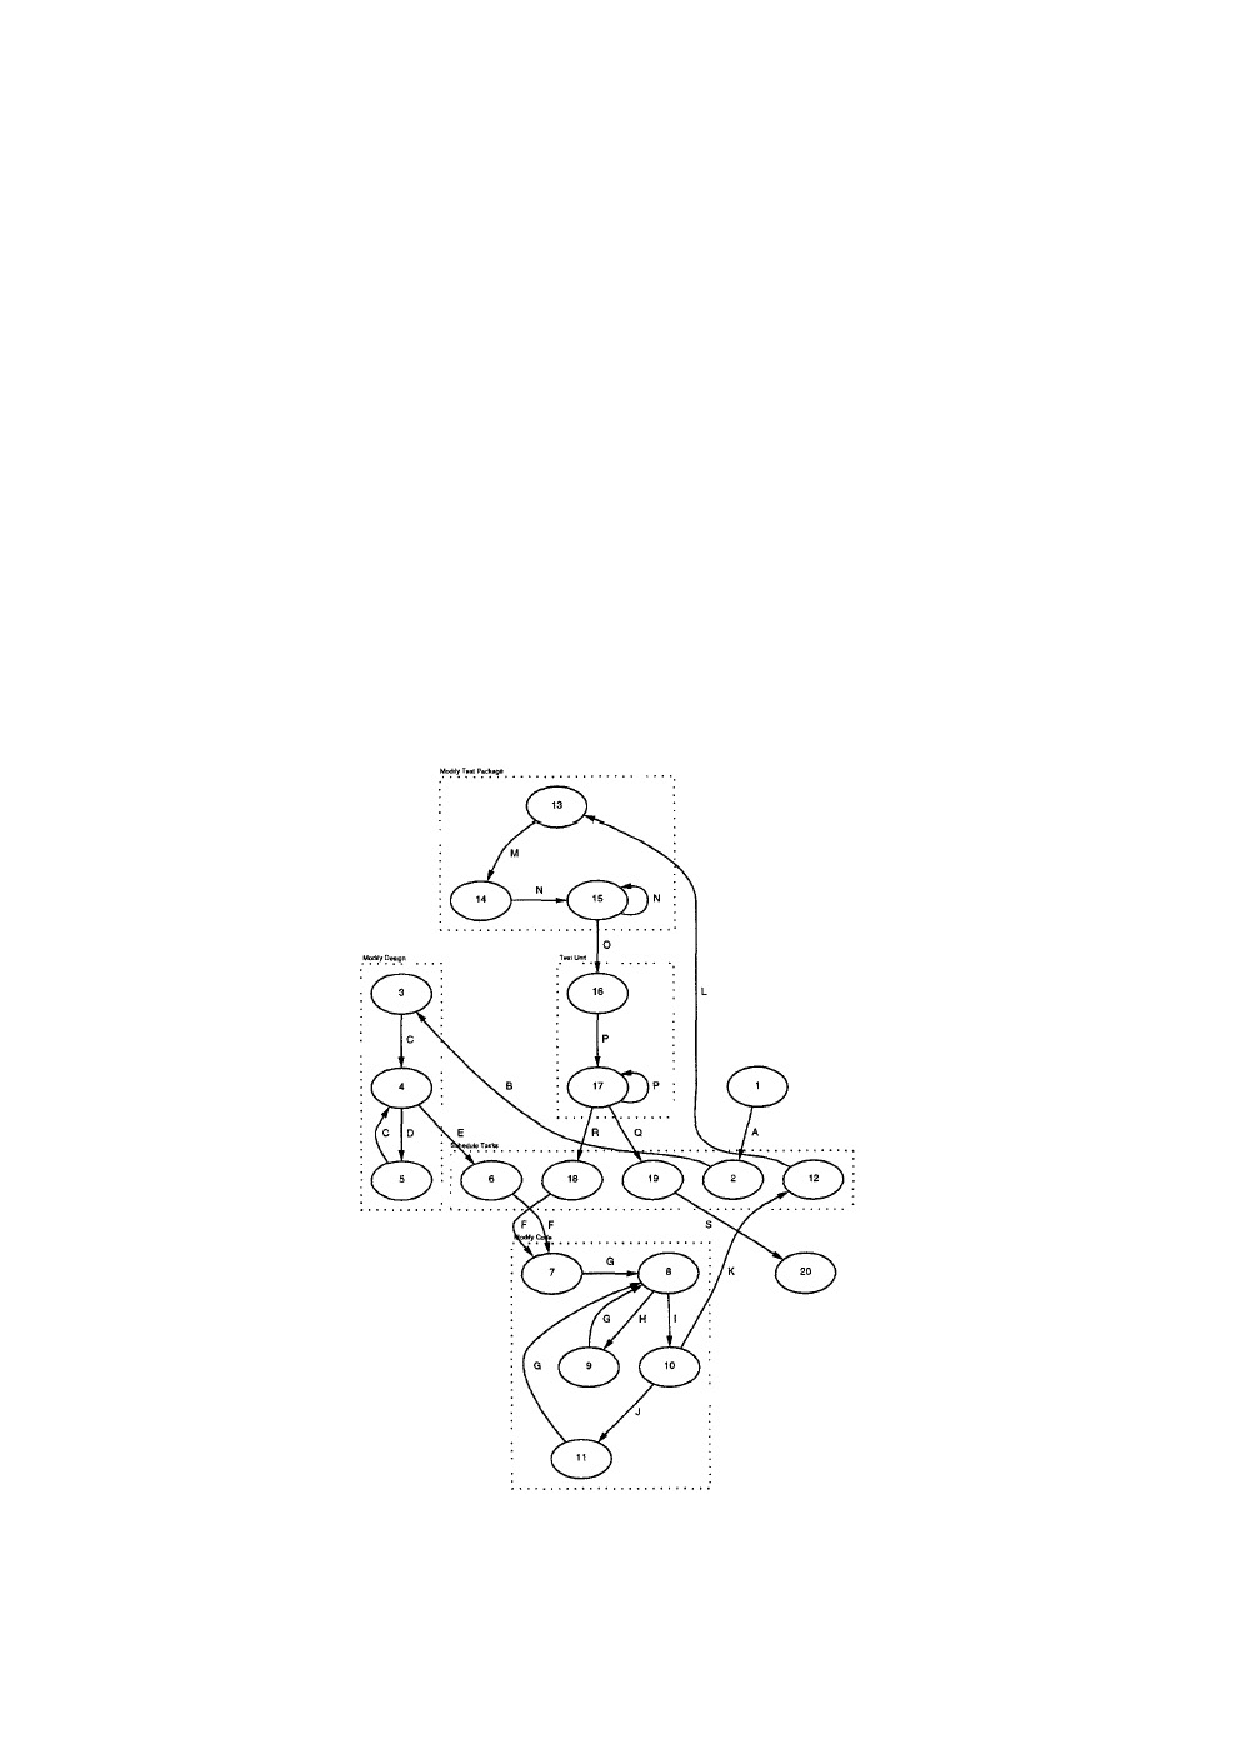
\includegraphics[width=0.6\textwidth]{figs/Balboa}
  \caption{Discovery of ISPW 6/7 Process (MARKOV )\cite{Cook:95}}
  \label{fig:Balboa}
\end{figure}
The numbered circles in Figure \ref{fig:Balboa} are the process 
states, and the arrows represent the development event data. 
Although Cook demonstrated that the generated FSM in Figure 
\ref{fig:Balboa} is very close to the actual ISPW 6/7 process, 
FSM does not look like an ideal technique for automated process
discovery and validation. The process FSM can be too complicated
to be useful. In \cite{Cook:95}, the three algorithms RNET, KTAIL
and MARKOV generated 15, 20 and 25 states respectively, and the 
states are interwoven in complicated manners as shown in Figure 
\ref{fig:Balboa}. It is very hard to interpret the monolithic 
state chart without a thorough understanding of Balboa and the 
adopted software process.

\begin{comment}
The FSM illustrated in Figure \ref{fig:Balboa} was generated 
from a event stream with only 32 events :
\mbox{ABCDCEFGHGIJGIKLMNOPRFGIKLMNOPQS}.
To discover the process hidden in this event steam, RNET 
took 10.4 hours, KTAIL took 29.4 seconds, and the MARKOV 
model used 0.6 seconds on a Sparc 2 Sun workstation. 
\end{comment}

\subsection{Discovering and Modeling Open Source Software Processes}
Jansen and Scacchi \cite{Jensen:04,Jensen:05} simulated an 
automated approach to discover and model the open source 
software development processes. They took advantage of prior 
knowledge to discover the software development processes by 
modeling the process fragments using a PML description. Their 
prototype simulation found that they could detect unusually 
long activities and problematic cycles of activities. They 
suggested that a bottom-up strategy, together with a top-down 
process meta-modeling is suitable for automated process 
discovery. But they don't have a working software system except 
for a prototype implementation of the ``requirement and 
release'' process of the open source project NetBeans.

\subsection{Discussion of Automated Process Conformance Research}
Automated process conformance is essentially about 
knowledge discovery and data mining, in which ordered 
data streams are processed to discover and classify 
naturally recurring patterns. 

Cook and Wolf used artificial neural network with RNET algorithm, 
MARKOV probability model with Bayesian 
learning algorithm, and KTAIL algorithm to mine the development 
event streams for discovering software processes \cite{Cook:95}. 
But generating a monolithic process model represented in FSM 
does not appear to be a very usable solution for process conformance 
validation of complicated software processes. In addition, 
generating FSM is very time consuming according to the 
performance report \cite{Cook:95}.

Jansen and Scacchi \cite{Jensen:04} modeled the requirement and 
release process of a large open source project using PML. They 
applied the modeled process to examine the development activities 
and behaviors. This bottom-up strategy, together with a top-down 
process meta-modeling, seems more plausible than FSM for dealing
with complicated development behaviors.  

In my thesis research, after researching the knowledge discovery
and data mining algorithms and techniques, I chose a rule-based
system to study process conformance of low-level software 
processes. Instead of asking process experts to inspect the
FSM of the executed process as Cook and Wolf did \cite{Cook:95}, 
I converted the process knowledge into a set of rules and used them 
to infer the software development behaviors. My method
is very close to Jansen's and Scacchi's approach \cite{Jensen:04} 
except that I used rules rather than PML for process descriptions. 

An intriguing phenomenon of automated software process research
is the scarcity of directly related literature work. Perhaps this 
is due to the difficulty of collecting the process execution data. 
Cook and Wolf ignored the problem of data collection in their 
research and claimed that it is site-specific \cite{Cook:95}. 
Jansen and Scacchi took advantage of rich information on the web 
and hypothesized that the proposed model can be used for the 
process deployment, validation and improvement \cite{Jensen:04}. 

Fortunately, with the development of sophisticated software 
metrics collection system such as Hackystat, software 
development data can be collected automatically and unobtrusively \cite{Hackystat,csdl2-01-12,csdl2-01-13,csdl2-02-07}. In my thesis 
research, based upon low-level development activities collected by 
Hackystat sensors, I conducted the research of the process conformance 
of Test-Driven Development. 

Wang and Erdogmus \cite{Wang:04} argued that the empirical research 
of TDD suffers from the construct validity problem (as is also the 
case in some other empirical software engineering research) because 
it lacks process conformance. They developed a prototype called 
``TestFirstGauge'' to study the process conformance 
of TDD by mining the in-process log data collected by Hackystat. 
TestFirstGauge aggregates software development data collected
by Hackystat to derive programming cycles of TDD. They used T/P ratio 
(lines of test code verse lines of production code), testing effort 
against production effort and cycle time distribution as the indicator 
of TDD process conformance. This project precedes the Zorro software 
system\cite{csdl2-06-02}, and in fact it stimulated our research interest 
in studying low-level software process conformance. Unlike the
prototype implementation of TestFirstGauge in VBA using an Excel
spreadsheet, Zorro is integrated into the Hackystat system for automation,
reuse, and flexibility using rule-based system \cite{Friedman-Hill:03}.

Similarly, Wege \cite{Wege:04} also focused on automated support of TDD
process assessment, but his work has a limitation in that it uses the CVS
history of code. Developers will not commit on-going project data at the
granularity of seconds, minutes or hours when they develop the software
system, making this data collection technique problematic for the purpose
of TDD inference. Collecting rapid low-level development activities is
a must in order to infer the low-level software process such as TDD
automatically.

%\subsection{Scientific Derivation and Simulation}

\section{Chapter Summary}

In this chapter, I introduced Test-Driven Development (TDD), a widely 
adopted core practice of Extreme Programming. The key characteristic
of TDD is to develop software by writing tests first. The software industry has 
widely adopted TDD and significant efforts have been put into it by 
practitioners (see Section \ref{sec:related-tdd}). Often, it is claimed 
that TDD can greatly help to improve software quality and developer 
productivity. The other claimed benefits of TDD include simple design, 
programmer confidence, and time 
saving on maintenance because less time is needed for bug hunting and 
debugging (see Section \ref{sec:related-tdd}). Much research work has been 
conducted on TDD about software quality and developer productivity 
(see Section \ref{sec:related-empirical}), but the research findings are 
divided. Interestingly, the research results are consistent
when the experiment settings were similar. A possible explanation 
for this phenomenon is process conformance, which is a construct validity
threat for the research findings (see Section \ref{sec:related-automation}). 

To address these problems and produce greater consistency in research 
results, I propose the automated process conformance inference with 
support from a rule-based system. In this chapter, I compared my research 
to Cook's automated process discovery and validation, Jansen's simulation 
of open source software project process, Wang's and Erdogmus's TestFirstGauge 
project, and Wege's automated support for process assessment in TDD 
(see Section \ref{sec:related-automation}).

\begin{comment}
Much of the research work on TDD suffers from the threat of ``construct
validity'' \cite{Wang:04} because of the what has been termed as the
``process conformance'' problem. Wang and Erdogmus defined process
conformance as the ability and willingness of the subjects to follow a
prescribed process.  Janzen warned that inability to accurately
characterize process conformance is harmful to TDD research
\cite{Janzen:05}: Many organizations might be using the methodology without
talking about it.  Others might claim to be using a methodology when in
fact they are misapplying it. Worse yet, they might be advertising its use
falsely.  Surveys might be conducted to gauge a method's usage, but often
only those who are much in favor or much opposed to the methodology will
respond.

A handful of research work has been done on software process validation
\cite{Cook:95,Jensen:05} and the process compliance of Test-Driven
Development \cite{csdl2-06-02,Wang:04,Wege:04}.  Cook and Wolf
\cite{Cook:95} developed a client-server software system called Balboa to
do process discovery and validation using a finite state machine (FSM).
Balboa collects developers' invocations of Unix commands and CVS commits to
learn the software process using FSM and machine learning techniques. Cook was 
able to reproduce the ISPW
6/7 process with Balboa in his research.  However, FSM does not look like
an ideal solution for process validation because of the complexity of the
process FSM it generates. In his example, the three algorithms RNET, KTAIL
and MARKOV generated 15, 20 and 25 states respectively, and the states are
interwoven in complicated manners. It is hard to interpret the process
state chart without thorough understanding of Balboa and the adopted
software process. Jansen and Scacchi \cite{Jensen:05} simulated an
automated approach to discovery and modeling of open source software
development processes.  They took advantage of prior knowledge to discover
the software development processes by modeling the process fragments using
a PML description. Their prototype simulation found that they could detect
unusually long activities and problematic cycles of activities. They
suggested that a bottom-up strategy, together with a top-down process
meta-modeling is suitable for automated process discovery. But they don't
have a working software system except for a prototype implementation.

Janzen \cite{Janzen:05} claimed that TDD is a kind of software development
method, not a process model, and that it has emerged out of a particular
set of process models. In contrast, Beck and Cunningham, the pioneers of
TDD, put it this way: ``test-first coding is not a testing technique but is
rather about design.''\cite{Beck:01} If TDD is a design technique and it
drives the implementation of product code, then classifying it as a
software process sounds reasonable. In my research, I have characterized
practices such as Test-Driven Development and Personal Software Process
(PSP) as low-level software processes. A common characteristic of a low-level
software process is that it is defined by many frequent and rapid
short-duration activities. Unlike high-level and long duration phases such
as ``requirement analysis'' that might last weeks to months, the activities
in low-level software process such as ``refactor class Foo to extract
interface IFoo'' may take only seconds to a few minutes \cite{csdl2-06-02}.

Low-level software processes often face similar research questions as
other, longer duration software processes. For instance, what process is
currently occurring, what process should occur, what are the impacts of a
given process on the important outcomes of software such as quality and
productivity, and how can a given process be improved and tailored in an
organization? So far, software engineering researchers have focused heavily
on the important outcomes that TDD brings to software products and software
developers. Both pedagogical
\cite{Muller:02,Edwards:04,Geras:04,Matjaz:03,Erdogmus:05,Kaufmann:03} and
industrial \cite{George:03,Maximilien:03,Bhat:06} evaluations of TDD have
been conducted in the last few years.  It is interesting to note that number of
research studies on TDD in academic settings is greater than the number of
research studies in industrial settings.

\section{Research Work in Academic Settings}
Most TDD research studies in academic settings seems to indicate that there
is some degree of quality improvement, but that there are little programmer
productivity benefits. Indeed, some studies have shown quality improvements
but at the cost of decreased productivity.

M\"{u}ller and Hanger \cite{Muller:02} conducted a study in an XP class in
Germany to test TDD in isolation of other XP practices against traditional
programming.  The acceptance tests were provided to both the TDD group and
the control group. Interestingly, students in the TDD group spent more time
but their programs were less reliable than the control group.  

Edwards \cite{Edwards:04} adopted TDD in a junior-level class to compare
whether students got more reliable code after the use of TDD and WEB-CAT,
an assignment submission system. It turned out that the students using TDD
reduced their defect rate dramatically (45\% fewer defects/KSLOC using a
proxy metric) after adopting TDD, and a posttest survey found that TDD
students were more confident of the correctness and robustness of their
programs.

Geras, Smith and Miller \cite{Geras:04} also isolated TDD from other XP
practices, and investigated the impact of TDD on developer productivity and
software quality. In their research, TDD does not require more time but
developers in TDD group wrote more tests and executed them more frequently,
which may have led to future time savings on debugging and development.

Pan\v{c}ur,Ciglari\v{c},Trampu\v{s}, and Vidmar \cite{Matjaz:03} designed 
a controlled experiment to compare TDD with Iterative Test-Last approach (ITL), 
which is a slightly modified TDD development process in the order of 
``code-test-refactor''.  This study found that TDD is somewhat different from 
ITL but the difference is very small.

A more recent study on the effectiveness of TDD conducted by Erdogmus,
Morisio and Torchiano \cite{Erdogmus:05} used the well-defined test-last
and TDD approaches as Pan\v{c}ur et al. did in \cite{Matjaz:03}. This study concluded
that TDD programmers wrote more tests per unit of programming effort. More
test code tends to increase software quality. Thus, TDD appears to improve
the quality of software but TDD group in the study did not achieve better
quality on average than test-last group.

Kaufmann \cite{Kaufmann:03}'s pilot study on implications of TDD, in
contrast, reported improved software quality and programmers' confidence.

\section{Research Work in Industrial Settings}
Several attempts have been made by researchers to study software quality
and productivity improvements of TDD in industrial settings.  

George and Williams \cite{George:04} ran a set of structured experiments
with 24 professional pair programmers in three companies. Each pair was
randomly assigned to a TDD group or a control group to develop a bowling
game application. The final projects were assessed at the end of the
experiment.  They found that TDD practice appears to yield code with
superior external code quality as measured by a set of blackbox test cases,
and TDD group passed 18\% more test cases. However, the TDD group spent
16\% more time on development, which could have indicated that achieving
higher quality requires some additional investment of time. Interestingly,
and in the contrast to the empirical findings, 78\% of the subjects
indicated that TDD practice would improve programmers' productivity.

Maximilien and Williams \cite{Maximilien:03} transitioned a software team
from an ad-hoc approach to testing to TDD unit testing practice at IBM, and
this team improved software quality by 50\% as measured by Functional
Verification Tests (FVT).

Another study of TDD at Microsoft conducted by Bhat and Nagappan
\cite{Bhat:06} reported remarkable software quality improvement as measured
in number of defects per KLOC. After introducing of TDD, project A
(Windows) reduced its defects rate by 2.6 times, and project B (MSN)
reduced its defect rate by 4.2 times, compared to the organizational
average. Reportedly, developers in project A spent 35\% more development
time, and developers in project B spent 15\% more development time, than
the developers in non-TDD projects spent.

\section{Process Conformance Study of TDD}
As we can see from the literature, there are discrepancies in the empirical
findings across both educational settings and industrial settings. Sometimes the
discrepancies are dramatic, for example \cite{Muller:02} found that the TDD
group yielded less reliable programs than the control group, while
\cite{Bhat:06} reported that the TDD group improved software quality by 
over four times.

Wang and Erdogmus \cite{Wang:04} pointed out there are several
possibilities that might explain why there are the discrepancies in TDD
research findings. For example, discrepancies could occur due to
differences in populations, differences in teaching methods and materials,
and differences in the techniques by which TDD is compared. They argued
that TDD empirical software research lacks process conformance, and
therefore it suffers from the construct validity problem (as is also the
case in some other empirical software engineering research). In
\cite{Wang:04}, they developed a prototype called TestFirstGauge to study
the process conformance of TDD by mining the in-process log data collected
by Hackystat. TestFirstGauge aggregates software development data collected
by Hackystat to derive programming cycles of TDD. They use T/P ratio (lines
of test code verse lines of production code), testing effort against
production effort and cycle time distribution as the indicator of TDD
process conformance. This project precedes the Zorro software system
\cite{csdl2-06-02}, and in fact it stimulated our research interest in
studying low-level software process conformance. Unlike the
prototype implementation of TestFirstGauge in VBA using an Excel
spreadsheet, Zorro is integrated into the Hackystat system for automation,
reuse, and flexibility using rule-based system \cite{Friedman-Hill:03}.

Similarly, Wege \cite{Wege:04} also focused on automated support of TDD
process assessment, but his work has a limitation in that it uses the CVS
history of code. Developers will not commit on-going project data at the
granularity of seconds, minutes or hours when they develop the software
system, making this data collection technique problematic for the purpose
of TDD inference.
\end{comment}